% Read takeover timing after a T-Bit of 1, styled after Figure 2.1.
% Only the controller-facing signals are shown.
\begingroup
\sffamily
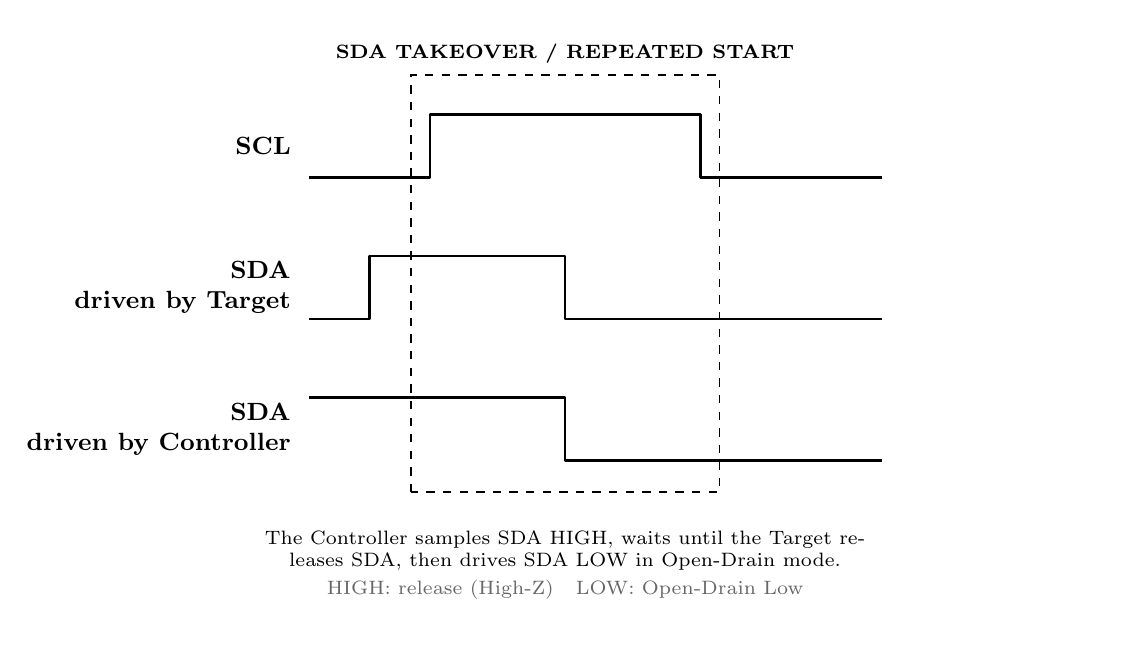
\begin{tikzpicture}[
    xscale=0.70,
    font=\small,
    wave/.style={draw=black, line width=1pt, line join=round},
    window/.style={draw=black, dashed, line width=0.6pt},
    hiddenevent/.style={draw=black!55, dotted, line width=0.6pt},
    siglabel/.style={font=\small\bfseries, anchor=east, align=right},
    condlabel/.style={align=center, font=\scriptsize\bfseries, text=black},
    note/.style={align=center, font=\scriptsize, text=black},
  ]

  % Takeover window: SCL is held HIGH while ownership returns to Controller.
  \draw[window] (1.85,0.75) rectangle (7.45,6.05);

  % SCL: extended high phase gives the Target time to release SDA.
  \draw[wave]
    (0,4.75) -- (2.20,4.75) -- (2.20,5.55)
    -- (7.10,5.55) -- (7.10,4.75) -- (10.40,4.75);

  % SDA driven by Target: T=1 is HIGH before the Target releases SDA.
  \draw[wave]
    (0,2.95) -- (1.10,2.95) -- (1.10,3.75)
    -- (4.65,3.75) -- (4.65,2.95) -- (10.40,2.95);

  % SDA driven by Controller: remains released until the Target release time has elapsed.
  \draw[wave]
    (0,1.95) -- (4.65,1.95) -- (4.65,1.15) -- (10.40,1.15);

  \node[siglabel] at (-0.15,5.15) {SCL};
  \node[siglabel] at (-0.15,3.35) {SDA\\driven by Target};
  \node[siglabel] at (-0.15,1.55) {SDA\\driven by Controller};

  \node[condlabel] at (4.65,6.32) {SDA TAKEOVER / REPEATED START};

  \node[note, anchor=north, text width=10.2cm] at (4.65,0.38)
    {The Controller samples SDA HIGH, waits until the Target releases SDA, then drives
     SDA LOW in Open-Drain mode.\\[2pt]
     {\color{black!60}HIGH: release (High-Z)\quad LOW: Open-Drain Low}};

  % Keep the shortened SCL-high interval centered with safe margins for the labels.
  \pgfresetboundingbox
  \path[use as bounding box] (-5.10,-0.90) rectangle (14.40,6.65);
\end{tikzpicture}
\endgroup
